\documentclass[11pt]{article}


\usepackage{setspace}
\doublespace
\usepackage{multicol}
\usepackage{parskip}
\usepackage{titlesec}
\usepackage[section]{placeins}
\usepackage{xcolor}
%\usepackage{breakcites}
\usepackage{lineno}
\usepackage{hyphenat}






\PassOptionsToPackage{hyphens}{url}
\usepackage[colorlinks = true,
            linkcolor = blue,
            urlcolor  = blue,
            citecolor = blue,
            anchorcolor = blue]{hyperref}
\usepackage{etoolbox}
\makeatletter
%\patchcmd\@combinedblfloats{\box\@outputbox}{\unvbox\@outputbox}{}{%
%  \errmessage{\noexpand\@combinedblfloats could not be patched}%
%}%
\makeatother


\usepackage{natbib}




\renewenvironment{abstract}
  {{\bfseries\noindent{\abstractname}\par\nobreak}\footnotesize}
  {\bigskip}

\titlespacing{\section}{0pt}{*3}{*1}
\titlespacing{\subsection}{0pt}{*2}{*0.5}
\titlespacing{\subsubsection}{0pt}{*1.5}{0pt}


\usepackage{authblk}


\usepackage{graphicx}
\usepackage[space]{grffile}
\usepackage{latexsym}
\usepackage{textcomp}
\usepackage{longtable}
\usepackage{tabulary}
\usepackage{booktabs,array,multirow}
\usepackage{amsfonts,amsmath,amssymb}
\providecommand\citet{\cite}
\providecommand\citep{\cite}
\providecommand\citealt{\cite}
% You can conditionalize code for latexml or normal latex using this.
\newif\iflatexml\latexmlfalse
\providecommand{\tightlist}{\setlength{\itemsep}{0pt}\setlength{\parskip}{0pt}}%

\AtBeginDocument{\DeclareGraphicsExtensions{.pdf,.PDF,.eps,.EPS,.png,.PNG,.tif,.TIF,.jpg,.JPG,.jpeg,.JPEG}}

\usepackage[utf8]{inputenc}
\usepackage[ngerman,english]{babel}



\usepackage{float}








\begin{document}

\title{the acoustic correlates of vowel prominence in concord/conflict at song/syllable
levels: Estonian~\emph{regilaul} folksong meter\emph{.}}




\author[]{sally ransom}%
\affil[]{University of Texas at Austin}%


\vspace{-1em}



  \date{\today}


\begingroup
\let\center\flushleft
\let\endcenter\endflushleft
\maketitle
\endgroup


\bigskip
\begin{quote}\begin{center}
{\it I don't use folksongs, \\
rather,\\
folksongs use me}\\
-Veljo Tormis, Estonian composer and {\it regilaul} revitalist
\end{center}
\end{quote}


\titlepage





\sloppy







\section*{Abstract}

 This corpus phonetics study of Estonian folk songs examines vowel space and duration in conflict and concordance at the song and the syllable-levels of prosodic prominence. Songs are useful for examining acoustic correlates of stress because they are restricted in the domain of time, having less temporal variation than natural ``running" speech. By examining the interaction of temporal and spatial acoustic cues in various positions, we can see how a singer accomodates prosodic conflicts to preserve contrasts in the language. The paper first introduces prosodic prominence in general, then delves into the metrical specifics of Estonian and its folksong tradition. After outlining the research questions, the methods section describes the corpus of {\it regilaul}: its construction, annotation, and processing. Results show that for vowel duration, * is the best predictor of vowel length. In the spatial domain, however, * is the best predictor of vowel length.
 
  \section*{Introduction}

At the interface of language and music is the lyrical song, with natural language participating in the musical domain as the (adjective) resonator for the vocal instrument. In this domain we can examine the effects of the musical context on the language: while bpm varies naturally in human performances, phrases in musical contexts are more consistent than in running speech \cite{}. Both music and language share the notion of rhythmic prominence, with certain beats (or syllables) carrying extra weight or ``stress."  \\

A primary focus of research in metrical prosody is the acoustic properties of stress or prominence at different levels of the prosodic heirarchy and its bounds. In a language, syllables have a prominence status at every level: every foot has a strongest syllable, each word has a strongest foot, each clause a strongest word, and on and up. When lyrics are put to a melody, an additional level is added to the prosodic hierarchy, this one with heavy restrictions in the temporal domain, subordinating all lower prosodic levels to that of the song. \\

This paper takes the interface of music and language as an opportunity for an exploratory corpus phonetics study of syllable prominence using the Estonian language, which has three syllable quantities, a predictable stress pattern at the word level and a robust tradition of folksongs {\it regilaul} which follow a strict metrical pattern. \\

\subsection*{Acoustic Prominence} 
 
 At present, typological data shows that across languages, syllable prominence is indicated by a convergence of several cues: i.e.,  duration, spectral balance, vowel space, and onset consonant length \cite{sluijterSpectralBalanceAcoustic1996,gordonPHONETICCORRELATESSTRESS1997, libermanStressLinguisticRhythm1977,berinsteinWPPNo471979,dejongStressLexicalFocus2004}.
Syllable prominence can also be thought of as localized hyperarticulation \cite{dejongSupraglottalArticulationProminence1995}. It is well documented that speakers spontaneously adjust the articulatory and acoustic dimensions of their speech to a given context, i.e., when communicating to someone who is hard of hearing, to an L2 speaker, or in a noisy restaurant. \cite{smiljanicbradlow}. In these situations, certain acoustic dimensions are exaggerated: expanding the vowel space, lengthening certain duration cues, increasing the intensity of certain frequencies \cite{}. Conversely, in facilatory situations such as speaking to someone very familiar, the opposite (hypo articulation) happens, where certain acoustic elements are diminished. \cite{lindblomExplainingPhoneticVariation1990}. Decades since H \& H theory, an abundance of research has shown gradient acoustic effects of speech modification. Rather than a manner of speaking in [plusminus] difficult context, we see a convergence of cue weighting and adjustments along a several continua of contexts.  \\
 
We can think of strong syllables as hyperarticulated compared to their weaker (hypoarticulated) peers, with the strongest syllable at the highest level the most hyperarticulated compared to its strong peers. \\

 
% Estonian’s stress pattern in well established: it is a trochaic language, with a foot consisting of a stressed syllable followed by one or more unstressed syllables. Its secondary stress falls iteratively on odd-numbered syllables\cite{lehisteFunctionQuantityFinnish1965}. Stress in natural Estonian words always falls on the first syllable. Estonian {\it regilaul} songs use what is known as the Kalevala meter, each verse has eight syllables with iterative trochaic stress. The question at hand is: what are the acoustic results of conflict between word and song prominence?
 

 When a listener hears a syllable in some sort of conflict, such as word-stressed but song-unstressed, they may or may not perceive it as conflicting or concordant. However, we might assume the singer's production to contain acoustic evidence of the conflict if they are a native speaker of the language they are singing. The null hypothesis is that song and word-level prominent syllables are no different from each other: that is, the highest prosodic hierarchy in this case the song) will dominate prominence in the temporal domain, confirming the earlier Ross \& Lehiste studies where a syllable's position in the song's metrical pattern is the best predictor for syllable duration.   \\
Temporal and spectral correlates of prominence: \\ 

\subsection*{Stress in Estonian}

Syllables in Estonian have three quantities, resulting in three types of durationally contrastive feet, so that the same bisyllabic sequence can mean three different things depending on the quantity. \cite{rossTimingEstonianFolk1998}.
 \begin{figure}[htbp]
 \begin{center}
 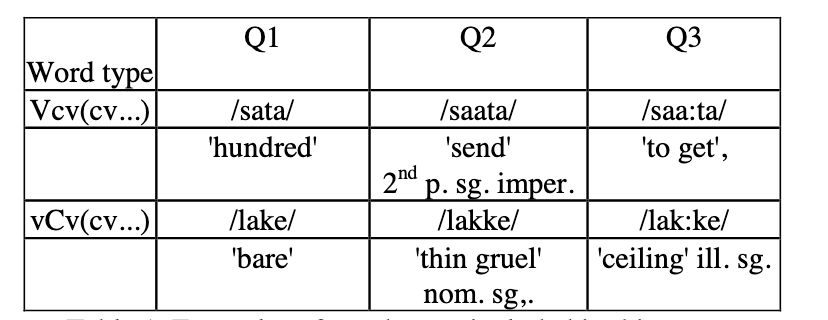
\includegraphics[width=200pt]{figures/Quantity.png}\\

 \caption{Three Way Quantity Contrast {(\it Krull, 1999)}}
 \label{quant_cont}
 \end{center}
 \end{figure}
 
 There is a documented tendency for foot isochrony, a consistency in duration of feet in Estonian which results in an inverse relationship between the durations of the two syllables in a foot: the longer the first syllable, the shorter the second. This is realized acoustically by the duration ratio of first and second syllable in a foot, i.e., second syllables that follow an overlong syllable will be realized shorter than a second syllable that follows a long syllable. \\
 \begin{itemize}
 	\item Q1 – short 		ratio ~2/3	(short-long(er))
	\item Q2 – long		ratio ~3/2	(long(er)-short(er))
	\item Q3 – overlong		ratio ~2/1 	(long(er)-short(er)) 
\end{itemize}
 
  In list reading speech, the duration ratio is greater between short and long syllables, but in conversational speech this is only seen in situations where the bearer of quantity contrast is a vowel, and f0 is available as a secondary cue for quantity. In conversational speech when the contrast bearer is a consonant, the duration ratio is greater between long and overlong syllables. 
 \\

 With few exceptions, such as in borrowed words, Estonian stress is predictable from the following rules:
 \begin{itemize}
 	\item if the syllable is in the third quantity, stress falls on its nucleus. 
	\item otherwise, primary word stress is on the first syllable. 
\end{itemize}
%
%It has also been proposed that some overlong syllables may constitute a monosyllabic foot all on their own (Hint 1973), (Prince, 1980).

Estonian is mostly trochaic, with main stress falling on the first syllable and secondary stress falling iteratively on odd-numbered syllables \cite{lehisteFunctionQuantityFinnish1965}. 
In other words, a left-edge, quantity sensitive iterative stress pattern.
\subsection*{Kalevala Meter}
  The Kalevala meter is part of the musical tradition of both Estonia and Finland. The main element in the structure of the songs is the verse line, consisting of eight positions divided between four (usually trochaic) feet. From the point of view of musical rhythm, the majority of old folksong melodies are roughly isochronous, i.e. consisting of notes of about the same
 duration. In most cases, each of the eight positions holds one syllable for one melody note. As an exception, two syllables may fit one note, or a syllable (usually a diphthong) may be divided between two notes. This is readily evident in the musical score, which is divided into four or eight. Ictus refers to a position that is stressed in a song, and off-ictus is an unstressed position in a song. In {\it regilaul} songs, which make use of the Kalevala meter, the pattern is trochaic: ictus starts on the first beat and is applied to every other syllable of a phrase. \\
 
 
 \begin{figure}[htbp]
\begin{center}

\includegraphics[width=300pt]{melody.png}
\caption{one {\it regilaul} phrase in music notation}
\label{default}
\end{center}
\end{figure}





 
[...]
\subsection*{Previous Work}
%What happens, then, when a trisyllable (which should have S w S pattern at the word level) is followed by, say, a bisyllable (assuming only Q1 and Q2 for this simple example) with the pattern S w, but has to be fit into the strict trochaic kalevala meter? Will the trisyllable present as a dactyl /S.w.w/ followed by a more faithful trochee in the bisyllable S.w? Or will the trisyllable remain faithful as /S.w.S/, forcing the bisyllabic following sequence to surface as /w.S/? In either result, what are the acoustic modifications made by the performer: does the song-level stress dominate the dimension of time (e.g. duration lengthens for all ictus positions) while word-level prominence is still negotiated by another acoustic correlate of stress?  \\

  A previous study in Estonian \cite{rossTradeoffQuantityStress1996} found that duration was a better predictor of musical verse position than of word stress: stressed syllables in off-ictus lost their durational contrast with unstressed syllables. When syllable duration is subordinated to the song meter, what acoustic modifications does the singer make to preserve word stress?
A previous study \cite{rossTradeoffQuantityStress1996} examined the relationship of the conflict between word stress and metrical ictus (stress position in the song), finding that word-level duration cues were subordinated to the musical prominence pattern. \\

 Another study,
 \cite{rossLostProsodicOppositions1994} compared S1/S2 ratios for all three quantity degrees in three Estonian funeral laments, finding that duration was best predicted by metrical position and not syllable quantity. 
 \cite{rossTradeoffQuantityStress1996}
 Syllables in ictus position were longer than syllables in off-ictus position
 measured syllable duration ratios (S1/S2) for two categories of Q1 (short) words: those with initial syllable(which would be stressed in speech) falling in ictus position and with initial syllable falling in off-ctus position (resulting in a conflict between word stress and metrical ictus). They found that the duration ratios of Q1 words that started in ictus was greater than that which started in off-ictus. Q1 words starting in ictus position tended to have notes of approximately the same duration, while those that started in off-ictus position tended to shorten the initial syllable.  \\

More recent work has found that proportional duration increases \cite{Lunden} between adjacent syllables is a more robust metric than simple duration ratio. This paper aims to extend and increase the {\it n} of the aforementioned studies of these songs' prosodic hierarchies by annotating a larger corpus of {\it regilaul}, to compare measurements of syllable duration ratios and proportional duration differences of syllable quantity and prominence in songs. \\

The extension of the findings arises after confirming the duration results. If duration is not the contrastive cue for syllable stress or quantity in songs, what (if any) are the acoustic cues for syllable prominence and quantity contrast? Therefore in addition to duration, vowel space and spectral tilt will be  measured in syllable vowel nuclei.


 If duration is subordinated to the prosody of the music, we can predict that another cue to linguistic stress will be retained in the singer’s production: for this paper, we will look at vowel quality. 

\subsection*{Research Questions and Hypotheses}

 The hypothesis is that stressed syllables that fall in off-ictus positions will be have raised intensity in higher frequency bands \cite{sluijterSpectralBalanceAcoustic1996} due to constricted vocal folds, and  will be hyperarticulated \cite{lindblomExplainingPhoneticVariation1990} compared to unstressed syllables in those same positions. 

% 
%  In Estonian, stressed syllables tend to have a higher pitch than the following syllable. Will the singer adjust the melody when a stressed word falls in an off-ictus position, to avoid it being lower than the following (weak) syllable? 

 \begin{itemize}
 \item Stressed syllables that fall in off-ictus positions will be hyperarticulated (higher high vowels, lower low vowels) compared to unstressed syllables in those same positions. 

 \item Duration will be subordinated to metrical structure, so vowel duration will be predicted more accurately by song position than word stress. 

 \item Stressed syllables in off-ictus positions will have an increase in intensity at higher frequencies than unstressed syllables in those same positions. 
 \end{itemize}
 

[...]
\section*{Methods}
This section is outlined as follows: first, the corpus of {\it regilaul} songs is described in detail, including information about the archival source and collectors, the performers in the recordings, text transcriptions of the lyrics, and the digital audio signal. Then, the annotation methods for phrase, beat, word, syllable, and segment are demonstrated, proceeding finally to the acoustic measurements.

\subsection*{Materials}



% all parnumaa

% a total of thirty-two minutes, twelve seconds of recorded song
% seven singers 

% ages 67 to 92, average age 75 years old
% all women


% Three singers ()
% all were recorded within the same five year time span in the 1960s in Parnumaa county by a total of three different female singers.


The Anthology of Estonian Traditional Music \hyperref[csl:1]{(Tampere, n.d.)}provides an overview of the earlier folk music tradition of Estonia, providing a sample of lyrics, English translations, and archival audio (.ogg) recordings of 98 {\it regilaul} songs and 17 instrumental tunes collected and compiled across Estonia's many parishes by Herbert Tampere, Erna Tampere, Ottilie K\selectlanguage{ngerman}õiva between 1912 and 1966 for the Estonian Folklore Archives in Tartu, Estonia. \\

For this project, a sample of 9 {\it regilaul} songs were chosen by the following criteria: all were recorded between 1960 and 1965 (likely with same or similar equipment) in the same region (Parnumaa, which according to an informant is a dialect with the aforementioned stress pattern). The singers were three women aged 67 and 92 (avg 75) years, and long-time residents of Parnumaa county at the time of the recordings. 

%Combined, the audio corpus totals thirty-two minutes and twelve seconds of recorded audio consisting mostly of songs with some running speech. 



% The chosen songs were also glossed word by word with the help of a native Estonian speaking consultant, who in turn helped determine word boundaries and word-play tokens, as well as providing some historical context.
%refine compression lossiness language, describe archive license and permissions,



\subsection*{Preparing Audio} 
%TODO cite sox
After downloading from the archive, the files were converted from .ogg to .wav files  using sox, as PRAAT\cite{PRAAT} \hyperref[csl:2]{(Boersna, n.d.)} cannot read the null bytes contained in .ogg files. \\
\subsubsection{TEMPO MAPPING}
First, I used the flex tempo feature of Logic Pro X to find the best fit of beats and tempo, adjusting the map to fit the downbeat of each measure and fitting the variable notes in time. Using this map enabled me to make a metronome of sorts that followed the true tempo of the performance. This midi metronome was programmed to strike on the down beat and at every other syllable division (given the melody of the song in question). Song data is available in the appendix. This midi file was then trimmed to match the song file exactly, so that PRAAT could automatically annotate sounds and silences for each song based on its variable tempo metronome. This had the effect of marking every ictus syllable with a simple script. The textgrids from this script were then the basis for the analysis tiers: first, every eight beats is taken as a large phrase interval, its appropriate lyric line inserted. Using the built-in eSpeak forced-aligner for Estonian, phrases were annotated to words, checked for accuracy, and then annotated to segments. Ictus and off-ictus boundaries were adjusted during the segmentation process to match onsets and offsets. First and second syllable vowels were annotated to new tiers, and then the intersection of ictus and first syllable, ictus and second syllable, off-ictus and first syllable, and off-ictus and second syllable were taken for analysis. From this intersection, midpoint formant measurements were extracted, as well as spectral tilt. 



\begin{figure}[htbp]
		\begin{center}
			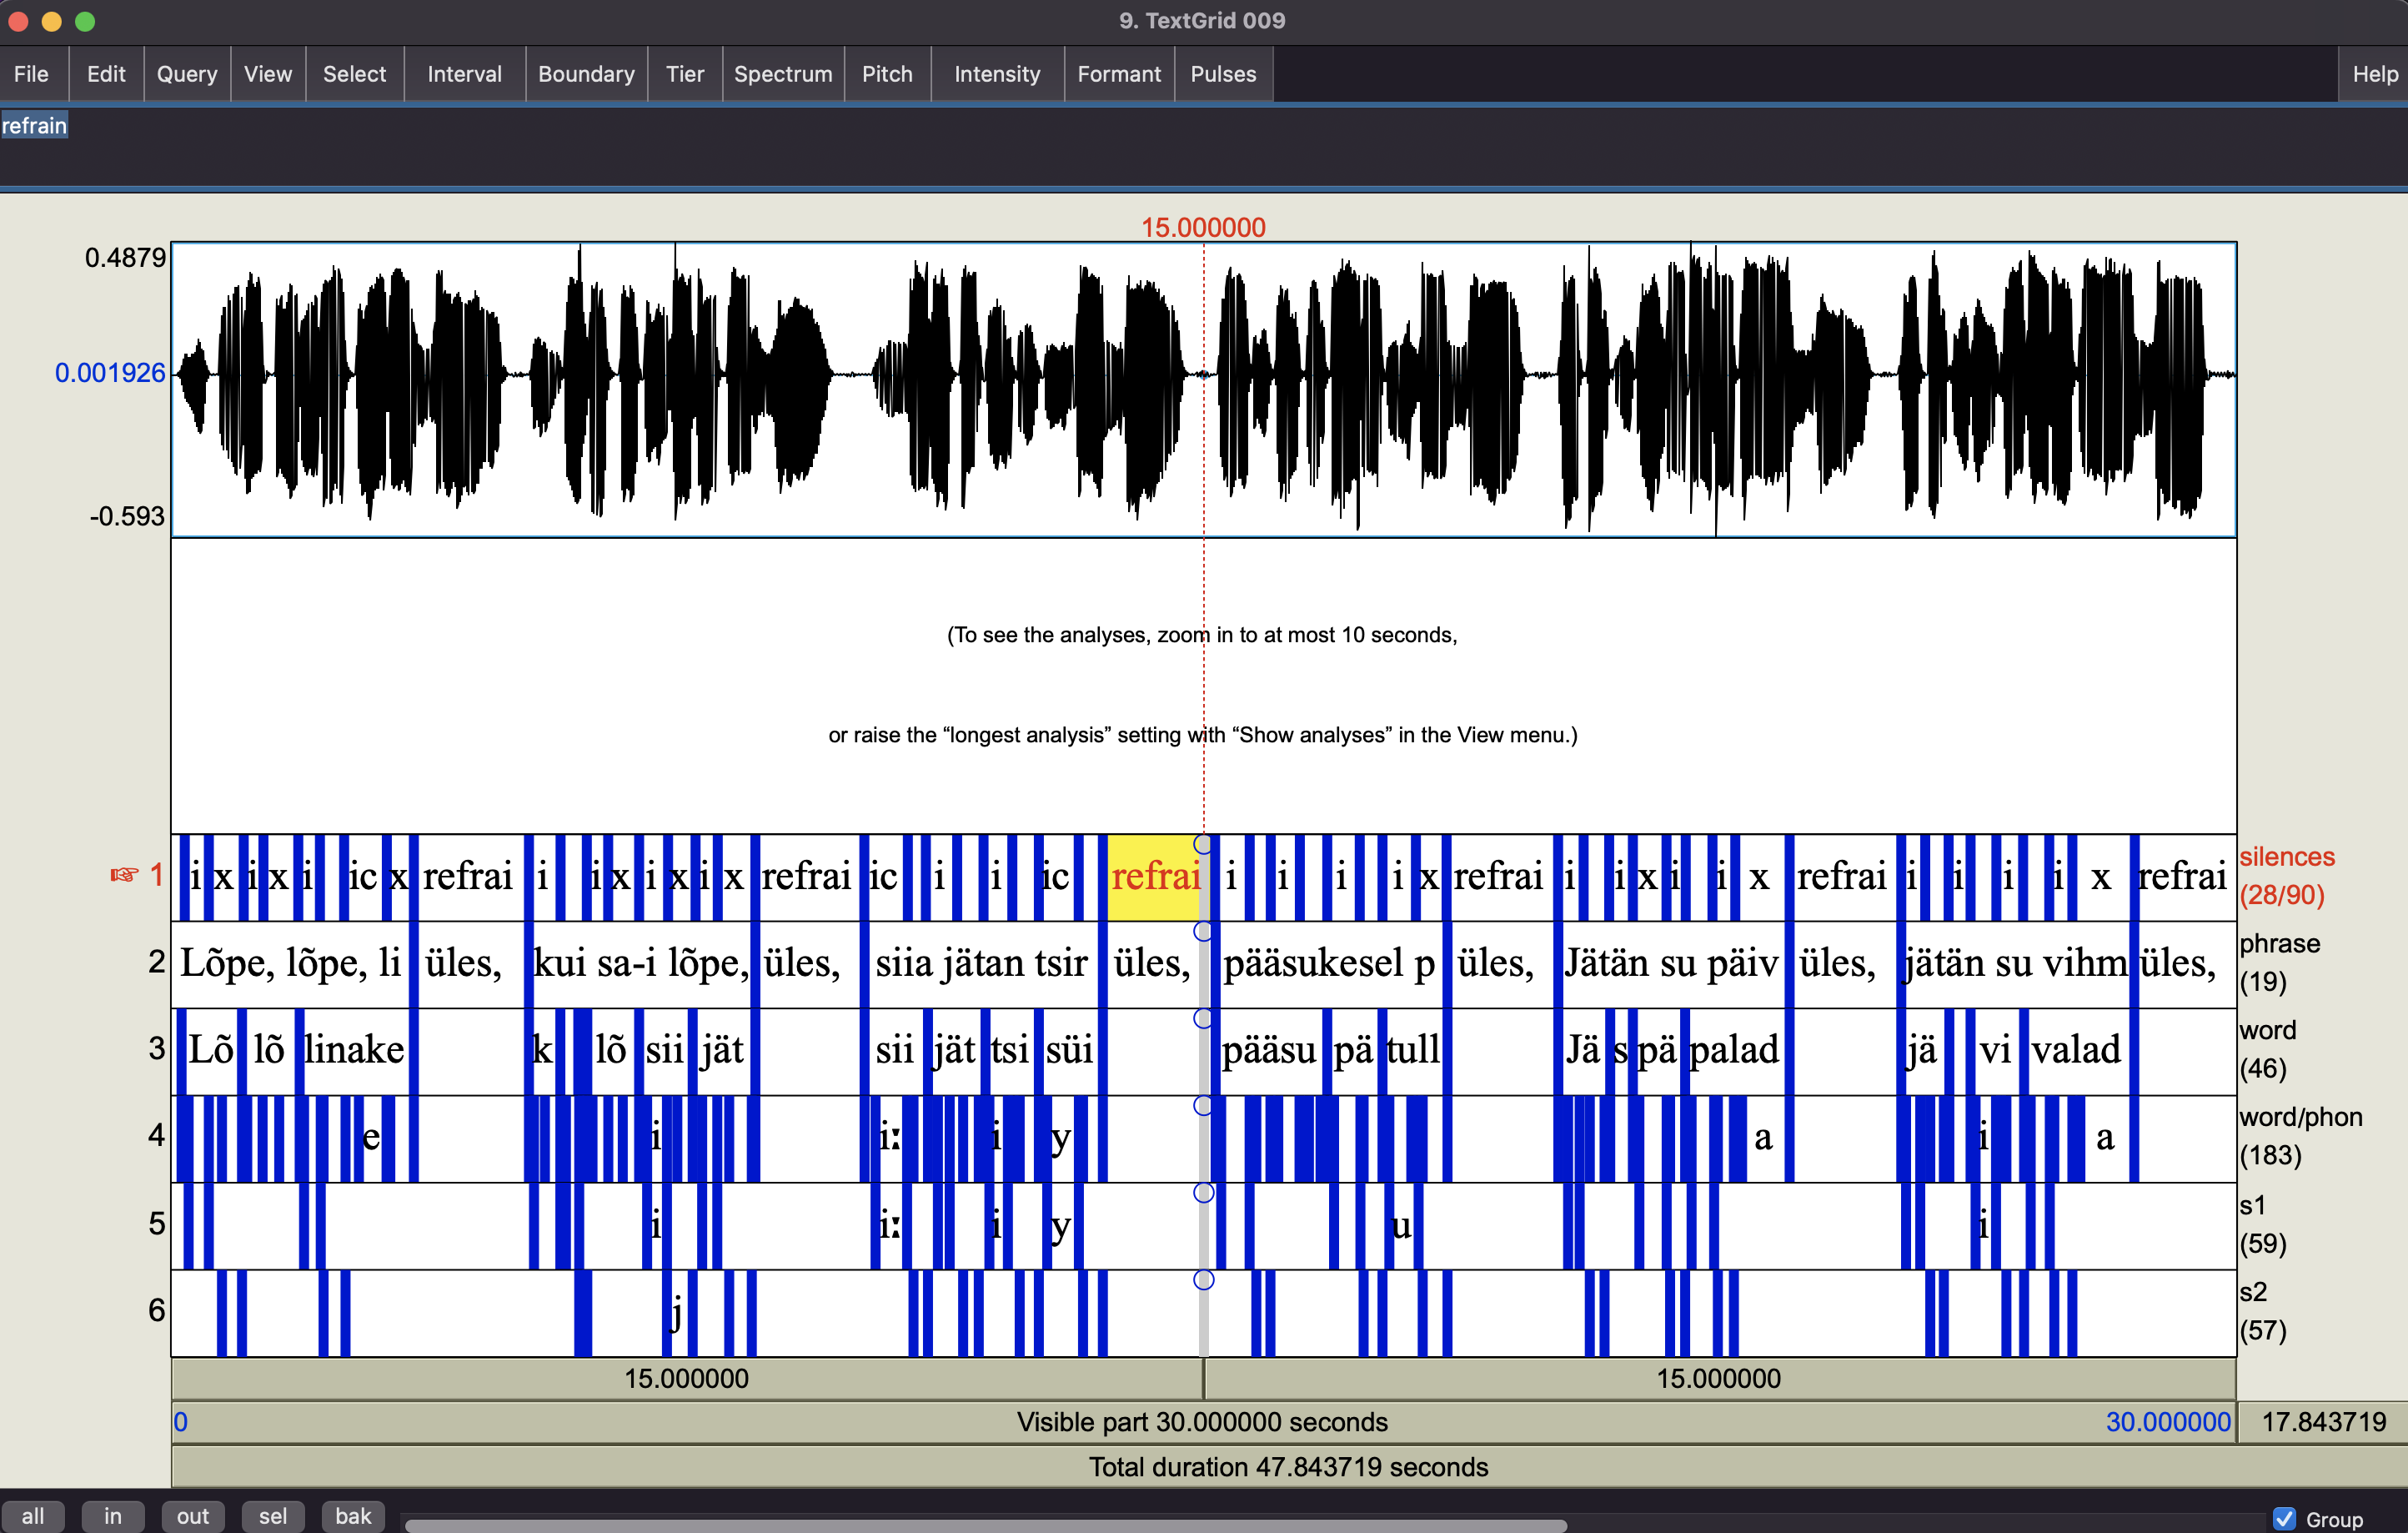
\includegraphics[width=300pt]{big_grid.png}
			
			\caption{whole song}
			\label{song_whole}
		\end{center}
	\end{figure}
		\begin{figure}[htbp]
\begin{center}
			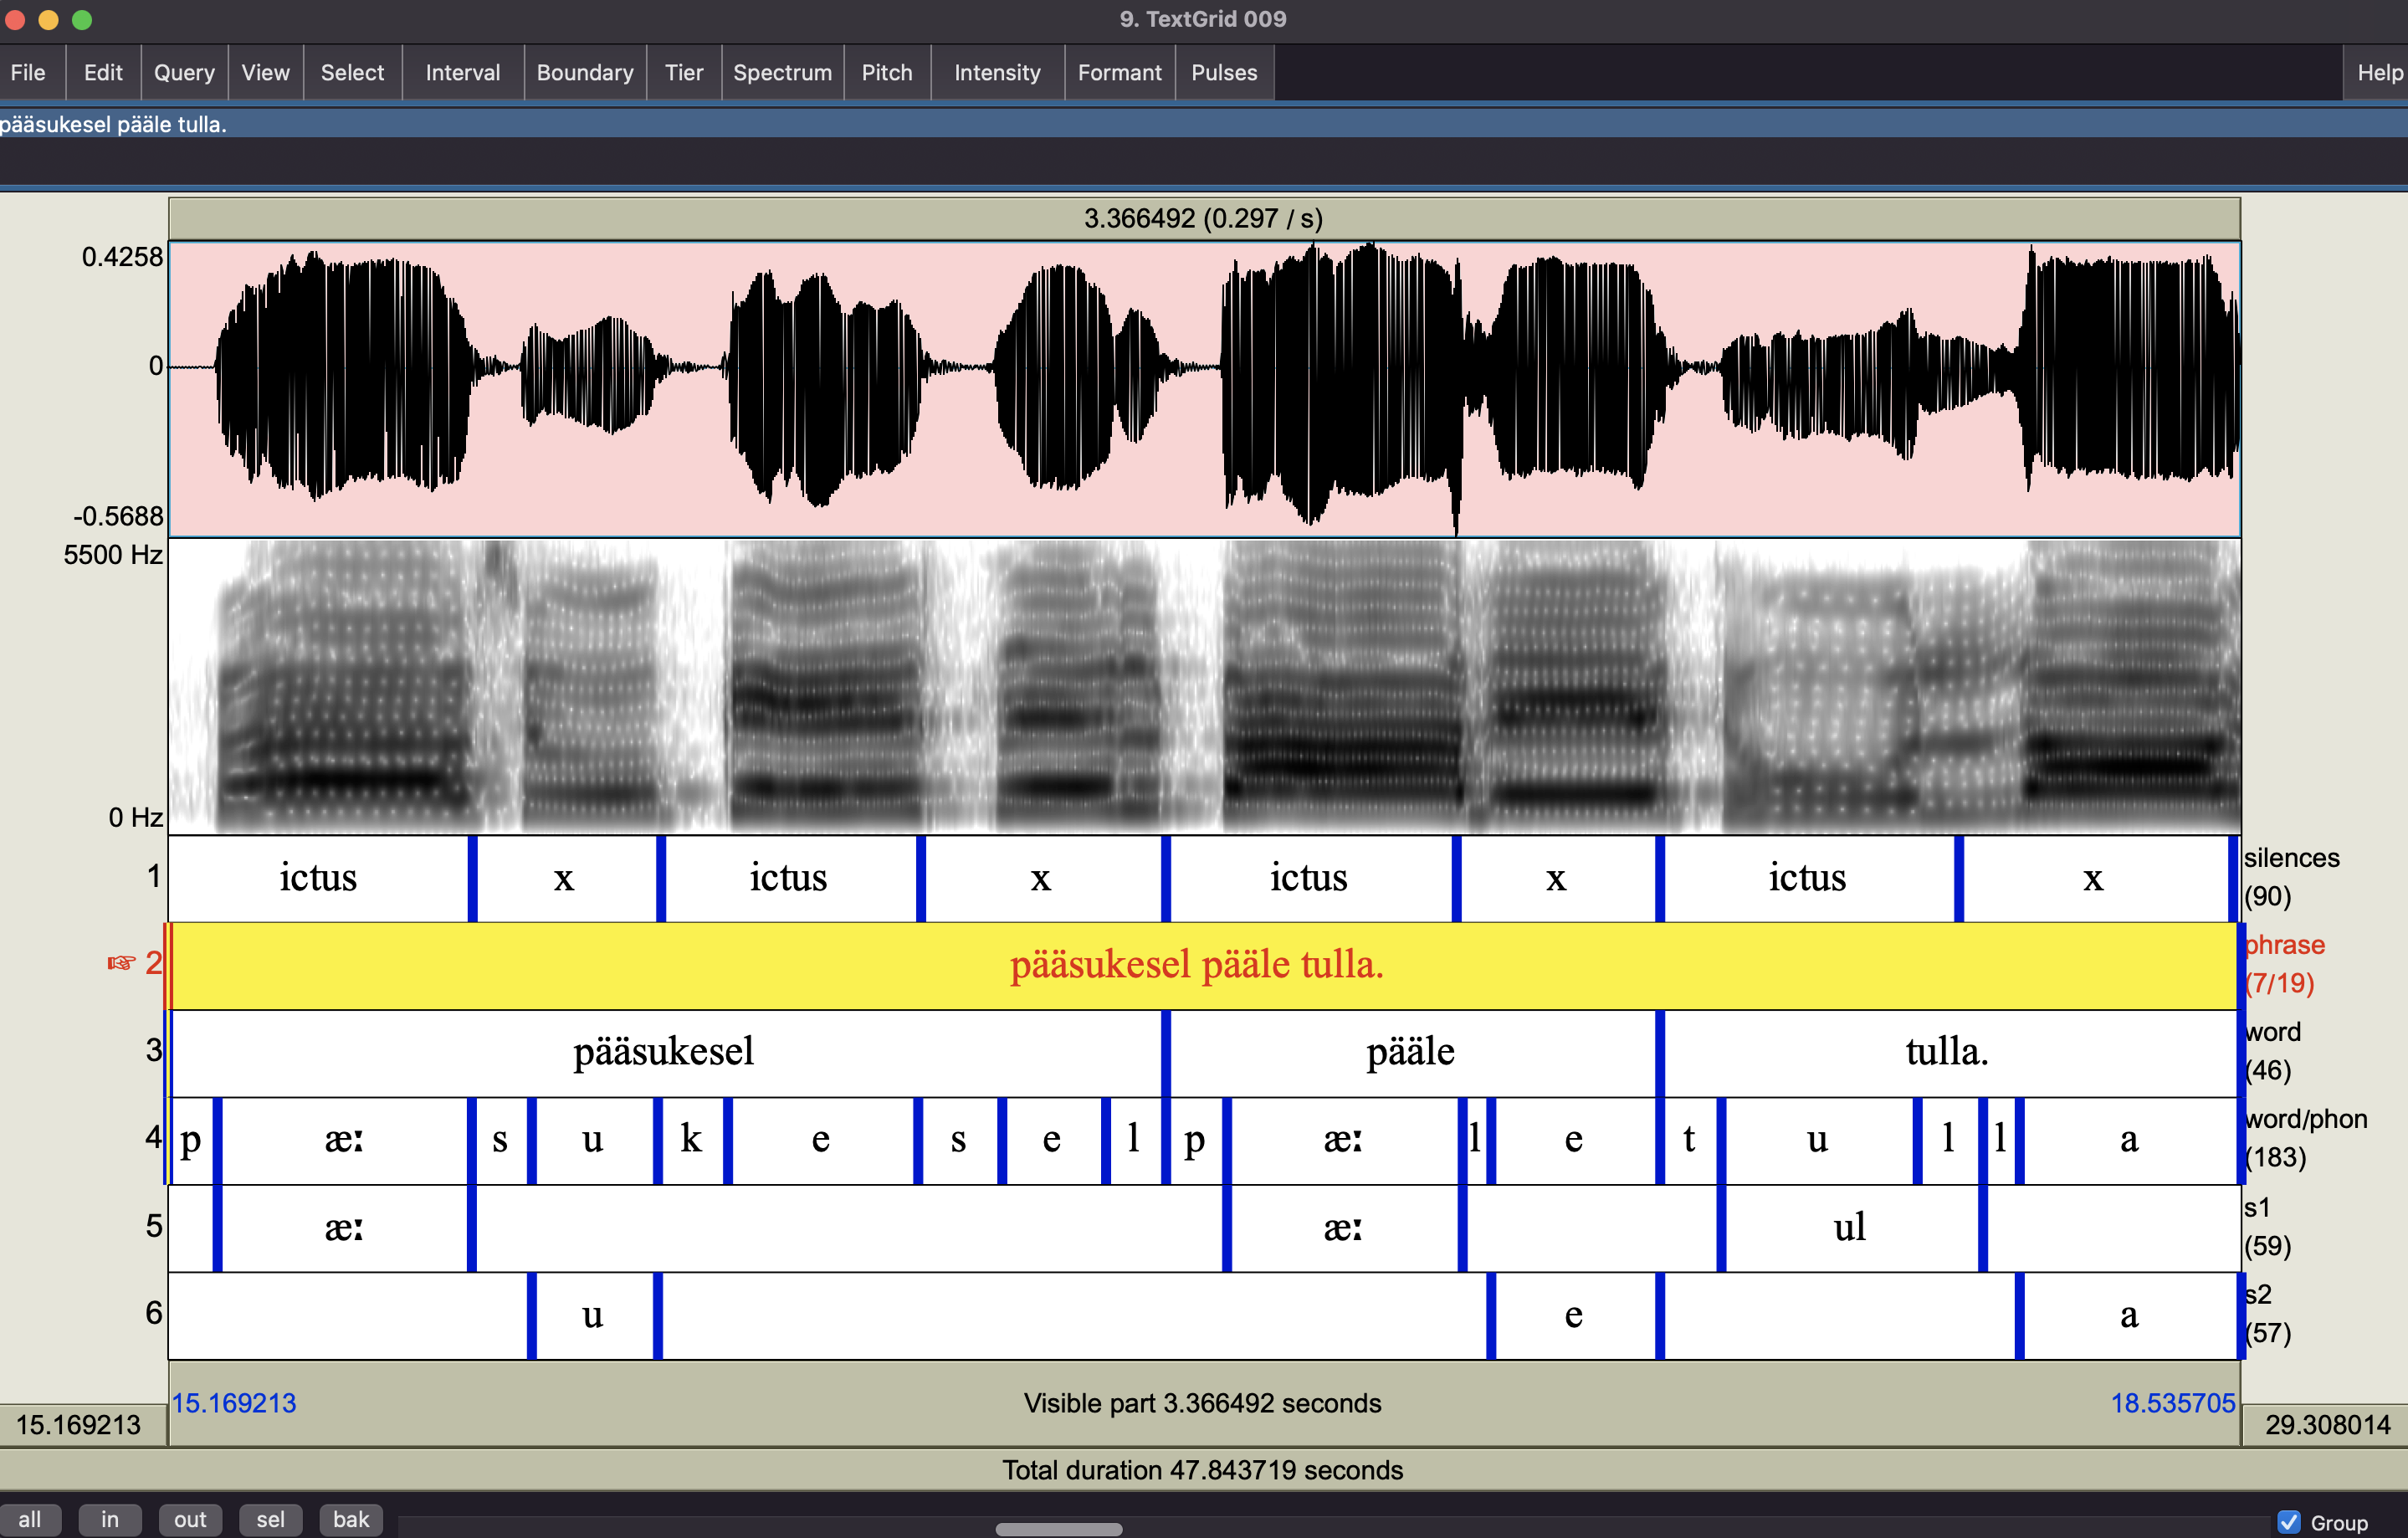
\includegraphics[width=300pt]{phrase_grid.png}
			\caption{single phrase}
\label{phrase}
\end{center}
\end{figure}

}


%TODO cite
%Each song is imported into Audacity\cite{}, where the Nyquist Beat detective plugin \cite{} is run with a sensitivity level of (25\%), generating a list of floats of the timepoints of detected points in the signal that are 25\% more prominent than the surrounding signal. This is used to create a point tier of each beat in a PRAAT Textgrid. The textgrids from this script were then the basis for the analysis tiers: first, every eight beats is taken as a large phrase interval, its appropriate lyric line (in Estonian orthograph) inserted into the Interval tier. After verifying the phrase intervals for each grid, PRAAT's built-in eSpeak forced aligner for Estonian is then iterated on each phrase to the word and phoneme level. Each tier is then manually checked by the author such that each annotation verifiably contains its labeled sound(s) and no other, otherwise it is excluded from measurements. \\
% that are adjacent to a pause, where a pause is considered a silent period of at least ()dB and ()ms long.
% Phrase boundaries are defined by the beats, which tend to fall on syllable nuclei. Oral stop consonants at phrase boundaries are ignored, as it is difficult to determine the boundary between silent events in acoustic data.  
\subsection*{Syllable Segmentation, Temporal and Spectral Measurement Criteria}

The following criteria were used to adjust the results of the forced aligner when the segment boundaries were verifiably off. \\
\subsubsection*{Segmental/Temporal}
onsets: \\

Oral stops at phrase boundaries are excluded. Due to the continuous nature of singing, most words with oral stop onsets have enough preceding acoustic energy to determine the boundary, but care is still taken to exclude stop consonants at word boundaries adjacent to pauses. 

%	\item for nasals, at the boundary of the anti-formants
vowels:\\
The criteria for a vowel onset following stop consonants is at the beginning of the release burst,
and at the clear increase in amplitude in the waveform and visible formants in spectrogram following other obstruents. Following nasals, vowel onset is defined at the boundary of detectible anti-formants. The boundaries of vowel onsets following liquids and glides are disregarded and instead these sequences are analyzed as a diphthong.

The criteria for the offset of a vowel preceding stop consonants is defined at the drop in acoustic energy upon closure preceding the small tail of f0 dropoff. Vowel offset preceding other obstruents is at the boundary between visible vowel formants and noisier acoustic energy, and for nasals at the boundary between vowel formants and antiformants. 
Preceding liquids and glides, no boundary is determined between vowel and coda, these are segmented with the vowel and analyzed as a diphthong. 
Long vowels are annotated as geminate, with the boundary between the two identical vowels being considered arbitrary, and the midpoint of the full double sequence used as the location of spectral measurements. 
coda: \\
liquid codas are included in total syllable duration, analyzed as a part of the vowel 



\subsubsection*{Spectral Measurement Parameters}
tilt, cog
[..]
%Diphthongs are excluded from formant measurements.
%\begin{table}[htp]
%\caption{formant analysis parameters:}
%\begin{center}
%\begin{tabular}{|l|l|}
%\hline
%
%time step: & 0.01s \\
%\hline
%max \# formants: & 5 \\
%\hline
%max Hz: & 5500 (adult female) \\
%
%\hline
%
%\end{tabular}
%\end{center}
%\label{default}
%\end{table}
%\item {\bf syllable coda criteria:} 
%	\begin{itemize} 
%		\item fricatives: 
%		\item for nasals, at the boundary between vowel formants and antiformants
%		\item 
%First and second syllable vowel segment boundaries were adjusted to meet the criteria and then copied to new respective tiers for analysis. Using praatio, we take the intersection of each possible song-ictus and word-stress position: 
%\begin{table}[htp]
%\caption{stress and ictus combinations}
%\begin{center}
%\begin{tabular}{|c|c|c|}
%\hline
% & ictus & off-ictus \\
%\hline
%strong & SS & SW*\\
%\hline
%weak &  WS* & WW \\
%\hline
%\end{tabular}
%\end{center}
%\label{strickTus}
%\end{table}%
%where (*) indicates a clash of song and word stress. For example, a stressed syllable in an off-ictus position is strong at the word level but weak at the song level. On the other hand, a strong syllable in ictus position has no clash, as it is strong at both the level of the word and the song. 
%
%
%\begin{enumerate}
%\item {\bf syllable onset criteria:}
%\begin{itemize} 
%	
%	
%	\end{itemize}
%\item {\bf syllable nuclei criteria:}
%\begin{itemize}
%	\item all vowels
%	\item long vowels analyzed as VV (only measured once)
%	\item liquid codas are analyzed as diphthongs
%	\item diphthongs are analyzed as VV, only measured for duration
%	\end{itemize}

%	\end{itemize}
%\end{enumerate}
\subsection*{Preparing Text}

The lyrics of each song are downloaded in a text file and aggregated into a corpus of songs together with annotated and transcribed audio. Using estnltk's Estonian toolkit, text data is used to filter and sort the acoustic data by quantity, syllable boundary, syllable-word index (i.e. stressed or not in speech) and syllable-phrase index (ictus or not at this metrical position in the song). 

\subsubsection*{syllabification}

At this point, the corpus is annotated for metrical position, phrase, word, and segment. However, in order to examine duration, a syllable quantity and stress annotation are necessary. Using an estonian version of nltk. \url{https://github.com/estnltk}, which has a useful automatic ``varbamorf"  syllabifier library. The output of the syllabification in this module includes syllable quantity and prominence data as well as the phoneme segments in each respective syllable. With the quantity annotated, duration measurements between syllable quantities can be compared with each other, to see if results are similar to \cite{rossTradeoffQuantityStress1996}.\\








%TODO add criteria! 

% At this point, the TextGrid contains four tiers: beats, phrases, words, and segments that have all been verified manually by the author. The word tier is now used as the scaffolding by which the estnltk \cite{} varbamorf \cite{} syllabification dictionary is created and added to the TextGrid. The dictionary contains a phonological transcription of each syllable, the quantity of the syllable (1, 2, or 3) and the stress status of the syllable, i.e., 1 for stressed syllables and 0 for unstressed. 




\section*{Results}

\subsection{Vowel Duration}

\subsection*{Vowel Space (F1 and F2)}

%introducing the graphs and the link to the notebook
%\begin{figure}[H]
%\begin{center}
%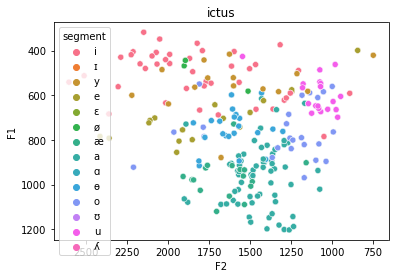
\includegraphics[width=0.70\columnwidth]{figures/ictus}
%\caption{{vowel chart for all vowels in ictus position
%{\label{198139}}%
%}}
%\end{center}
%\end{figure}\selectlanguage{english}
%\begin{figure}[H]
%\begin{center}
%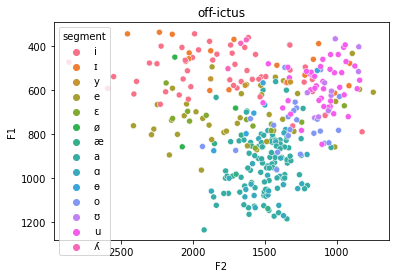
\includegraphics[width=0.70\columnwidth]{figures/off-ictus}
%\caption{{vowel chart for all vowels in off-ictus position
%{\label{146554}}%
%}}
%\end{center}
%\end{figure}
%
%
%\subsection*{Stressed and unstressed:\it{word-level prominence}}
%\subsection*{Vowel Space (F1 and F2}
%Introducing the graphs and the links\selectlanguage{english}
%\begin{figure}[H]
%\begin{center}
%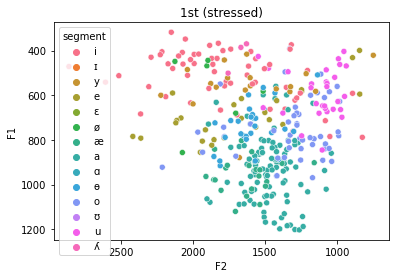
\includegraphics[width=0.70\columnwidth]{figures/first}
%\caption{{vowel space for stressed syllables
%{\label{216251}}%
%}}
%\end{center}
%\end{figure}\selectlanguage{english}
%\begin{figure}[H]
%\begin{center}
%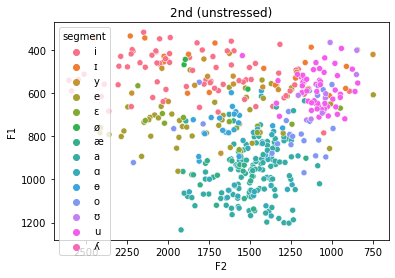
\includegraphics[width=0.70\columnwidth]{figures/second}
%\caption{{vowel space for unstressed syllables
%{\label{971548}}%
%}}
%\end{center}
%\end{figure}



%Introducing the graphs:
%\begin{figure}[H]
%\begin{center}
%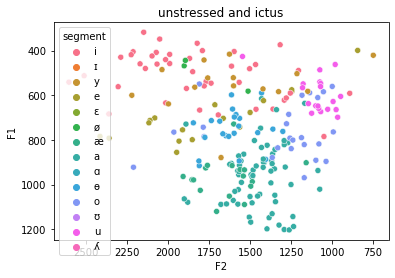
\includegraphics[width=0.70\columnwidth]{figures/unstressed-ictus}
%\caption{{Vowel Space of word-weak syllables in song-strong positions (conflicting
%prominence)
%{\label{632826}}%
%}}
%\end{center}
%\end{figure}\selectlanguage{english}
%\begin{figure}[H]
%\begin{center}
%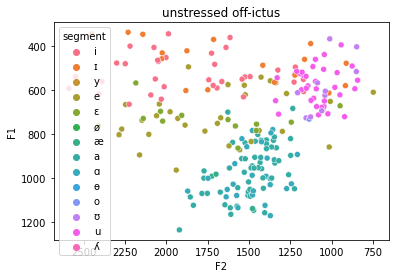
\includegraphics[width=0.70\columnwidth]{figures/unstressedoff-ictus}
%\caption{{Vowel Space of word-weak syllables in song-weak positions (concordant
%prominence)
%{\label{853436}}%
%}}
%\end{center}
%\end{figure}
%
%statistical analysis of word-weak combinations
%
%introducing the next graphs: song-strong conflicts\selectlanguage{english}
%\begin{figure}[H]
%\begin{center}
%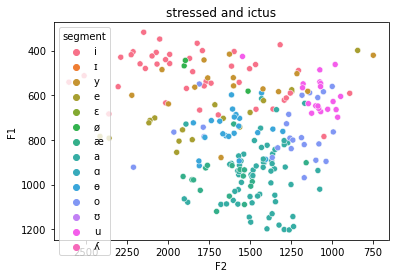
\includegraphics[width=0.70\columnwidth]{figures/stressed-ictus}
%\caption{{Vowel Space of word-strong syllables in song-weak positions (conflicting
%prominence)
%{\label{888534}}%
%}}
%\end{center}
%\end{figure}
%
%we'll say more things here
%\begin{figure}[H]
%\begin{center}
%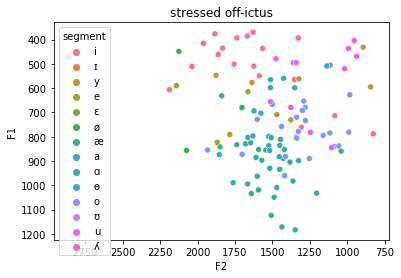
\includegraphics[width=0.70\columnwidth]{figures/stressedoff-ictus}
%\caption{{vowel space of word-strong syllables in song-weak positions (conflicting
%prominence)%
%}}
%\end{center}
%\end{figure}
%
%
%saying things \\

\section*{Discussion}
\subsection{Goin' Fishin' \n {\it some exploratory analysis I'd like to do with the data I've got}}

 Stress in Estonian is acoustically most often realized by onset consonant lengthening (Gordon, 1997; Hint, 1973). Gordon 1997 also found evidence for acoustic correlates of prosodic domains by measuring peak nasal flow, nasal amplitude, and duration in initial positions of four prosodic domains. The syllable, word, phrase, and utterance, were each also cross-classified for stressed and unstressed positions. \\
 
 
functional load hypothesis (Berinstein, 1979), \\
but another cross-linguistic study specifically analyzed the acoustic correlates of stress in languages that have a duration contrast, and found no support for the functional load hypothesis (Lunden et al., 2017). Thus this study has another potential theoretical bearing to weigh in on. 
\\
.The lowered amplitude of initial nasal segments (also found by (Fougeron 1996)), Gordon argues, is to maximize consonantness compared to the sonorance of the following vowel. Nasal data provided evidence for progressively larger domains of prosodic constituency: syllable, word, and phrase. 

Previous research has shown lengthening of domain-final segments (Oller 1973, Beckman et al 1992, Wightman et al 1992), wherein the higher the prosodic level, the greater the lengthening effect in general. Will this remain the case at different levels of the prosodic domain of the song?


\subsection{Syllable index within phrase compared to beats detected}
\begin{itemize}
\item rate of beats/syllables in each song
\item occurence of beats in odd (ictus) syllables
\item beats detected outside of ictus
\item overall robustness of the beat detection
\end{itemize}
\subsection{Duration Ratios:} \\


\subsubsection*{metrical analysis of text database of {\it regilaul}}
 a text database of {\it regilaul} songs: \url{https://www.folklore.ee/regilaul/andmebaas/?ln=en}. With this, I will analyze the frequency of stress and ictus conflicts in the larger pool of songs.  For example, are there more occurrences of syllables strong at the word level ending up in weak metrical positions, or more weak word-level syllables in strong metrical positions? How often do overlong (Q3, heaviest possible) syllables end up in metrically weak positions, if at all? \\
%In addition, looking forward to the future when I expand this corpus, I may strategize using the database to find songs that have several of the song and word stress conflicts that I am looking for. As these are folk songs, there will be multiple recordings of a given song, sometimes to different melodies or in different dialects. There would, of course, need to be a balance of songs where there are few or no conflicts to compare measurements to, but analyzing the database could also help to locate those. \\
At the very least, this database can provide some useful data, such as lexical frequency within the broader set of regilaul songs to provide a gradient picture of the present corpus in the context of {\it regilaul} songs on the whole. 

\subsection{Growing the Corpus} 
Available on the archive are eight more songs from the same region and time period, which would bring the total songs to 17 {\it regilaul} songs and seven singers. Once these annotations are aligned and verified, the audio corpus will total thirty-two minutes and twelve seconds of recorded audio. 

\section*{Conclusion}

[...]



%\section*{References}\sloppy
%\phantomsection
%\label{csl:1}\textit{{Anthology of {{Estonian Traditional Music}}}}. \url{https://www.folklore.ee/pubte/eraamat/rahvamuusika/en/index.}
%
%\phantomsection
%\label{csl:2}\textit{{Praat: Doing {{Phonetics}} by {{Computer}}}}. \url{https://www.fon.hum.uva.nl/praat/.}
\bibliographystyle{apalike}
\bibliography{QP.bib}
\end{document}

